\documentclass[11pt, letterpaper]{article}

% Fonts and Encoding
\usepackage[utf8]{inputenc}
\usepackage[T1]{fontenc}
\usepackage{lmodern} % High-quality Latin Modern vector font

% Math and Symbols
\usepackage{amsmath, amssymb, amsthm, amsfonts, mathrsfs, mathtools}

% Layout and Geometry
\usepackage{geometry}
\geometry{letterpaper, margin=1in}
\setlength{\parindent}{0pt}
\setlength{\parskip}{0.6em}

% Formatting and Graphics
\usepackage{graphicx, xcolor, enumitem, booktabs, array, tabularx}

% TikZ for Illustrations
\usepackage{tikz}
\usetikzlibrary{arrows.meta, positioning, shapes.geometric, calc, backgrounds, matrix}

% Clickable Links and TOC
\usepackage{hyperref}
\hypersetup{
    colorlinks=true,
    linkcolor=blue,
    filecolor=magenta,      
    urlcolor=cyan,
    pdftitle={Transforms of Discontinuous Functions},
}

% Theorem Environments
\newtheorem{theorem}{Theorem}[section]
\newtheorem{lemma}[theorem]{Lemma}
\newtheorem{proposition}[theorem]{Proposition}
\newtheorem{corollary}[theorem]{Corollary}
\theoremstyle{definition}
\newtheorem{definition}{Definition}[section]
\newtheorem{axiom}{Axiom}[section]
\newtheorem{example}{Example}[section]
\theoremstyle{remark}
\newtheorem{remark}{Remark}[section]

% Custom Commands (Enforced standard notation)
\newcommand{\R}{\mathbb{R}}
\newcommand{\N}{\mathbb{N}}
\newcommand{\Z}{\mathbb{Z}}
\newcommand{\Q}{\mathbb{Q}}
\newcommand{\E}{\mathbb{E}}
\newcommand{\Prob}{\mathbb{P}}
\newcommand{\F}{\mathcal{F}}
\newcommand{\Lap}{\mathcal{L}}

\begin{document}

\title{\textbf{Transforms of Discontinuous Functions}\\ \Large A Comprehensive Study Guide}
\author{Tashfeen Omran}
\date{\today}
\maketitle

\tableofcontents
\newpage

\section{Part 1: Comprehensive Introduction, Context, and Prerequisites}

\subsection{Core Concepts}
In the study of differential equations, we frequently encounter physical systems subjected to abrupt changes. A mechanical system might experience a sudden hammer strike, or an electrical circuit might have a switch flipped on and off. These sudden changes are modeled using \textbf{discontinuous functions}. The most fundamental building block for these functions is the \textbf{Heaviside Unit Step Function}, denoted as $u(t-a)$, which "turns on" at time $t=a$. 

By combining step functions, we can create \textbf{Rectangular Window Functions}, $\Pi_{a,b}(t) = u(t-a) - u(t-b)$, which turn a signal on at $t=a$ and off at $t=b$. The Laplace transform is uniquely powerful for solving differential equations with discontinuous forcing functions because it converts these piecewise functions into continuous algebraic expressions in the $s$-domain.

\subsection{Intuition and Derivation}
The Laplace transform of a function $f(t)$ is defined as $\Lap\{f(t)\} = \int_0^\infty e^{-st}f(t)\,dt$. 
If we apply this to the unit step function $u(t-a)$ (where $a \ge 0$):
\[
\Lap\{u(t-a)\} = \int_0^\infty e^{-st}u(t-a)\,dt = \int_a^\infty e^{-st}(1)\,dt = \lim_{N \to \infty} \left[ -\frac{e^{-st}}{s} \right]_a^N = \frac{e^{-as}}{s}
\]
This reveals a profound property: a delay in the time domain (shifting by $a$) corresponds to multiplication by an exponential factor $e^{-as}$ in the frequency ($s$) domain.

\subsection{Historical Context and Motivation}
Oliver Heaviside (1850–1925), an English electrical engineer, developed operational calculus to solve differential equations related to electrical circuits. He introduced the step function to model the switching of currents. Initially, mathematicians criticized his methods for lacking rigor, but his techniques were later fully justified by the formal development of the Laplace transform. Today, Heaviside's methods are indispensable in control theory, signal processing, and quantum mechanics.

\subsection{Key Formulas}
\begin{itemize}
    \item \textbf{Unit Step Function:} $u(t-a) = \begin{cases} 0, & t < a \\ 1, & t > a \end{cases}$
    \item \textbf{Rectangular Window:} $\Pi_{a,b}(t) = u(t-a) - u(t-b)$
    \item \textbf{Transform of Step:} $\Lap\{u(t-a)\} = \frac{e^{-as}}{s}$
    \item \textbf{Translation in $t$ (Second Shifting Theorem):} $\Lap\{f(t-a)u(t-a)\} = e^{-as}F(s)$
    \item \textbf{Practical Computation Form:} $\Lap\{g(t)u(t-a)\} = e^{-as}\Lap\{g(t+a)\}$
    \item \textbf{Inverse Translation:} $\Lap^{-1}\{e^{-as}F(s)\} = f(t-a)u(t-a)$
\end{itemize}

\subsection{Prerequisites}
To master this topic, you must be proficient in:
1. \textbf{Basic Laplace Transforms:} Knowing the transforms of $t^n$, $e^{at}$, $\sin(kt)$, and $\cos(kt)$.
2. \textbf{Partial Fraction Decomposition (PFD):} Essential for breaking down complex $s$-domain expressions.
3. \textbf{Completing the Square:} Required when dealing with irreducible quadratic denominators.
4. \textbf{Algebraic Shifting:} The ability to rewrite a function $g(t)$ in terms of $(t-a)$.

\newpage
\section{Part 2: Detailed Homework Solutions}
\textit{Note: The following solutions correspond to the Section 7.6 Exercises (Problems 1–36) from the provided text, which directly address the topic of Discontinuous Functions.}

\subsection{Problems 1–4: Sketch and Transform}

\textbf{Problem 1:} Sketch the graph and determine the Laplace transform of $(t-1)^2 u(t-1)$.
\\[4pt]
\textbf{Solution:}
The function is $0$ for $t < 1$ and follows the parabola $(t-1)^2$ for $t > 1$.
\begin{center}
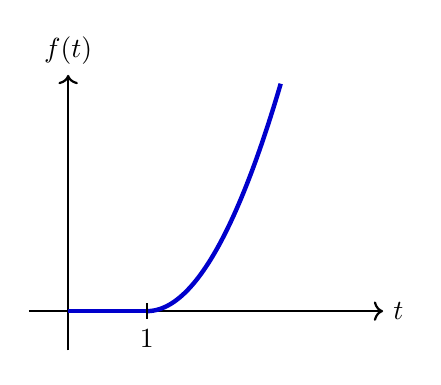
\begin{tikzpicture}[scale=1.0]
    \draw[->, thick] (-0.5, 0) -- (4, 0) node[right] {$t$};
    \draw[->, thick] (0, -0.5) -- (0, 3) node[above] {$f(t)$};
    \draw[ultra thick, blue!80!black, domain=1:2.7, samples=100] plot (\x, {(\x-1)^2});
    \draw[ultra thick, blue!80!black] (0,0) -- (1,0);
    \draw[thick] (1, 0.1) -- (1, -0.1) node[below] {$1$};
\end{tikzpicture}
\end{center}
Using the translation theorem $\Lap\{f(t-a)u(t-a)\} = e^{-as}F(s)$ with $f(t) = t^2$ and $a=1$:
\[
\Lap\{(t-1)^2 u(t-1)\} = e^{-s} \Lap\{t^2\} = e^{-s} \left( \frac{2}{s^3} \right) = \frac{2e^{-s}}{s^3}
\]

\textbf{Problem 2:} Sketch the graph and determine the Laplace transform of $u(t-1) - u(t-4)$.
\\[4pt]
\textbf{Solution:}
This is a rectangular window function $\Pi_{1,4}(t)$, which is $1$ between $t=1$ and $t=4$, and $0$ elsewhere.
\begin{center}
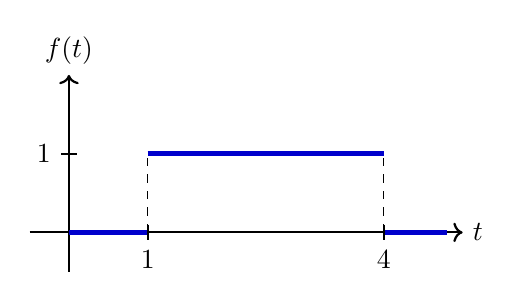
\begin{tikzpicture}[scale=1.0]
    \draw[->, thick] (-0.5, 0) -- (5, 0) node[right] {$t$};
    \draw[->, thick] (0, -0.5) -- (0, 2) node[above] {$f(t)$};
    \draw[ultra thick, blue!80!black] (0,0) -- (1,0);
    \draw[ultra thick, blue!80!black] (1,1) -- (4,1);
    \draw[ultra thick, blue!80!black] (4,0) -- (4.8,0);
    \draw[dashed] (1,0) -- (1,1);
    \draw[dashed] (4,0) -- (4,1);
    \draw[thick] (1, 0.1) -- (1, -0.1) node[below] {$1$};
    \draw[thick] (4, 0.1) -- (4, -0.1) node[below] {$4$};
    \draw[thick] (0.1, 1) -- (-0.1, 1) node[left] {$1$};
\end{tikzpicture}
\end{center}
Using the linearity of the Laplace transform:
\[
\Lap\{u(t-1) - u(t-4)\} = \frac{e^{-s}}{s} - \frac{e^{-4s}}{s}
\]

\textbf{Problem 3:} Sketch the graph and determine the Laplace transform of $t^2 u(t-2)$.
\\[4pt]
\textbf{Solution:}
The function is $0$ for $t < 2$ and jumps to the parabola $t^2$ for $t > 2$.
\begin{center}
\begin{tikzpicture}[scale=0.8]
    \draw[->, thick] (-0.5, 0) -- (4, 0) node[right] {$t$};
    \draw[->, thick] (0, -0.5) -- (0, 4) node[above] {$f(t)$};
    \draw[ultra thick, blue!80!black, domain=2:3, samples=100] plot (\x, {\x^2 - 2}); % Scaled for visual fit
    \draw[ultra thick, blue!80!black] (0,0) -- (2,0);
    \draw[dashed] (2,0) -- (2,2);
    \draw[thick] (2, 0.1) -- (2, -0.1) node[below] {$2$};
\end{tikzpicture}
\end{center}
We use the practical formula $\Lap\{g(t)u(t-a)\} = e^{-as}\Lap\{g(t+a)\}$. Here $g(t) = t^2$ and $a=2$.
\begin{align*}
g(t+2) &= (t+2)^2 = t^2 + 4t + 4 \\
\Lap\{t^2 u(t-2)\} &= e^{-2s} \Lap\{t^2 + 4t + 4\} = e^{-2s} \left( \frac{2}{s^3} + \frac{4}{s^2} + \frac{4}{s} \right)
\end{align*}

\textbf{Problem 4:} Sketch the graph and determine the Laplace transform of $t u(t-1)$.
\\[4pt]
\textbf{Solution:}
The function is $0$ for $t < 1$ and jumps to the line $y=t$ for $t > 1$.
\begin{center}
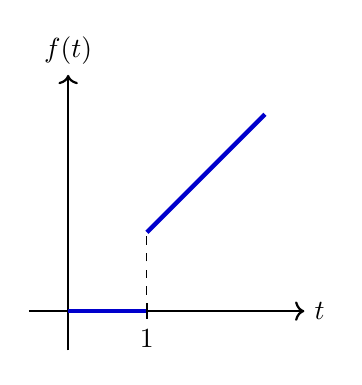
\begin{tikzpicture}[scale=1.0]
    \draw[->, thick] (-0.5, 0) -- (3, 0) node[right] {$t$};
    \draw[->, thick] (0, -0.5) -- (0, 3) node[above] {$f(t)$};
    \draw[ultra thick, blue!80!black] (0,0) -- (1,0);
    \draw[ultra thick, blue!80!black] (1,1) -- (2.5,2.5);
    \draw[dashed] (1,0) -- (1,1);
    \draw[thick] (1, 0.1) -- (1, -0.1) node[below] {$1$};
\end{tikzpicture}
\end{center}
Using $\Lap\{g(t)u(t-a)\} = e^{-as}\Lap\{g(t+a)\}$ with $g(t) = t$ and $a=1$:
\begin{align*}
g(t+1) &= t + 1 \\
\Lap\{t u(t-1)\} &= e^{-s} \Lap\{t + 1\} = e^{-s} \left( \frac{1}{s^2} + \frac{1}{s} \right)
\end{align*}

\subsection{Problems 5–10: Express using Window/Step Functions}

\textbf{Problem 5:} $g(t) = \begin{cases} 0, & 0 < t < 1 \\ 2, & 1 < t < 2 \\ 1, & 2 < t < 3 \\ 3, & 3 < t \end{cases}$
\\[4pt]
\textbf{Solution:}
We construct $g(t)$ by adding steps at each discontinuity:
\begin{align*}
g(t) &= 0 + (2 - 0)u(t-1) + (1 - 2)u(t-2) + (3 - 1)u(t-3) \\
g(t) &= 2u(t-1) - u(t-2) + 2u(t-3)
\end{align*}
Taking the Laplace transform:
\[
\Lap\{g(t)\} = \frac{2e^{-s}}{s} - \frac{e^{-2s}}{s} + \frac{2e^{-3s}}{s}
\]

\textbf{Problem 6:} $g(t) = \begin{cases} 0, & 0 < t < 2 \\ t+1, & 2 < t \end{cases}$
\\[4pt]
\textbf{Solution:}
\begin{align*}
g(t) &= (t+1)u(t-2)
\end{align*}
Using $\Lap\{f(t)u(t-a)\} = e^{-as}\Lap\{f(t+a)\}$:
\begin{align*}
f(t+2) &= (t+2) + 1 = t + 3 \\
\Lap\{g(t)\} &= e^{-2s}\Lap\{t+3\} = e^{-2s}\left(\frac{1}{s^2} + \frac{3}{s}\right)
\end{align*}

\textbf{Problem 7:} Graph shows $f(t) = t$ for $0 < t < 1$, and $f(t) = 1$ for $t > 1$.
\\[4pt]
\textbf{Solution:}
\begin{align*}
g(t) &= t(u(t) - u(t-1)) + 1u(t-1) = t - t u(t-1) + u(t-1) \\
g(t) &= t - (t-1)u(t-1)
\end{align*}
Taking the Laplace transform:
\[
\Lap\{g(t)\} = \frac{1}{s^2} - \frac{e^{-s}}{s^2}
\]

\textbf{Problem 8:} Graph shows $f(t) = \sin t$ for $0 < t < \pi/2$, and $f(t) = 0$ for $t > \pi/2$.
\\[4pt]
\textbf{Solution:}
\begin{align*}
g(t) &= (\sin t)(u(t) - u(t-\pi/2)) = \sin t - (\sin t)u(t-\pi/2)
\end{align*}
To transform $(\sin t)u(t-\pi/2)$, we shift the function: $f(t) = \sin t \implies f(t+\pi/2) = \sin(t+\pi/2) = \cos t$.
\begin{align*}
\Lap\{g(t)\} &= \Lap\{\sin t\} - e^{-\pi s / 2}\Lap\{\cos t\} = \frac{1}{s^2+1} - \frac{s e^{-\pi s / 2}}{s^2+1}
\end{align*}

\textbf{Problem 9:} Graph shows a triangle from $t=1$ to $t=3$, peaking at $(2,1)$.
\\[4pt]
\textbf{Solution:}
The line from $(1,0)$ to $(2,1)$ is $y = t-1$. The line from $(2,1)$ to $(3,0)$ is $y = -t+3$.
\begin{align*}
g(t) &= (t-1)\Pi_{1,2}(t) + (3-t)\Pi_{2,3}(t) \\
&= (t-1)[u(t-1) - u(t-2)] + (3-t)[u(t-2) - u(t-3)] \\
&= (t-1)u(t-1) - (t-1)u(t-2) + (3-t)u(t-2) - (3-t)u(t-3) \\
&= (t-1)u(t-1) - (2t-4)u(t-2) + (t-3)u(t-3) \\
&= (t-1)u(t-1) - 2(t-2)u(t-2) + (t-3)u(t-3)
\end{align*}
Taking the Laplace transform:
\[
\Lap\{g(t)\} = \frac{e^{-s}}{s^2} - \frac{2e^{-2s}}{s^2} + \frac{e^{-3s}}{s^2}
\]

\textbf{Problem 10:} Graph shows $f(t) = (t-1)^2$ for $t > 1$, and $0$ for $t < 1$.
\\[4pt]
\textbf{Solution:}
\begin{align*}
g(t) &= (t-1)^2 u(t-1) \\
\Lap\{g(t)\} &= e^{-s}\Lap\{t^2\} = \frac{2e^{-s}}{s^3}
\end{align*}

\subsection{Problems 11–18: Inverse Laplace Transforms}

\textbf{Problem 11:} $\Lap^{-1}\left\{ \frac{e^{-2s}}{s-1} \right\}$
\\[4pt]
\textbf{Solution:}
Let $F(s) = \frac{1}{s-1} \implies f(t) = e^t$. Using the inverse translation theorem:
\[
\Lap^{-1}\{e^{-2s}F(s)\} = f(t-2)u(t-2) = e^{t-2}u(t-2)
\]

\textbf{Problem 12:} $\Lap^{-1}\left\{ \frac{e^{-3s}}{s^2} \right\}$
\\[4pt]
\textbf{Solution:}
Let $F(s) = \frac{1}{s^2} \implies f(t) = t$.
\[
\Lap^{-1}\{e^{-3s}F(s)\} = (t-3)u(t-3)
\]

\textbf{Problem 13:} $\Lap^{-1}\left\{ \frac{e^{-2s} - 3e^{-4s}}{s+2} \right\}$
\\[4pt]
\textbf{Solution:}
Let $F(s) = \frac{1}{s+2} \implies f(t) = e^{-2t}$.
\begin{align*}
\Lap^{-1}\left\{ e^{-2s}F(s) - 3e^{-4s}F(s) \right\} &= f(t-2)u(t-2) - 3f(t-4)u(t-4) \\
&= e^{-2(t-2)}u(t-2) - 3e^{-2(t-4)}u(t-4)
\end{align*}

\textbf{Problem 14:} $\Lap^{-1}\left\{ \frac{e^{-3s}}{s^2+9} \right\}$
\\[4pt]
\textbf{Solution:}
Let $F(s) = \frac{1}{s^2+9} = \frac{1}{3} \frac{3}{s^2+3^2} \implies f(t) = \frac{1}{3}\sin(3t)$.
\[
\Lap^{-1}\{e^{-3s}F(s)\} = \frac{1}{3}\sin(3(t-3))u(t-3)
\]

\textbf{Problem 15:} $\Lap^{-1}\left\{ \frac{s e^{-3s}}{s^2+4s+5} \right\}$
\\[4pt]
\textbf{Solution:}
First, complete the square for the denominator: $s^2+4s+5 = (s+2)^2+1$.
Let $F(s) = \frac{s}{(s+2)^2+1} = \frac{s+2-2}{(s+2)^2+1} = \frac{s+2}{(s+2)^2+1} - \frac{2}{(s+2)^2+1}$.
The inverse transform is $f(t) = e^{-2t}\cos t - 2e^{-2t}\sin t$.
Applying the shift $t \to t-3$:
\[
\Lap^{-1}\{e^{-3s}F(s)\} = e^{-2(t-3)}(\cos(t-3) - 2\sin(t-3))u(t-3)
\]

\textbf{Problem 16:} $\Lap^{-1}\left\{ \frac{e^{-s}}{s^2+4} \right\}$
\\[4pt]
\textbf{Solution:}
Let $F(s) = \frac{1}{s^2+4} = \frac{1}{2} \frac{2}{s^2+2^2} \implies f(t) = \frac{1}{2}\sin(2t)$.
\[
\Lap^{-1}\{e^{-s}F(s)\} = \frac{1}{2}\sin(2(t-1))u(t-1)
\]

\textbf{Problem 17:} $\Lap^{-1}\left\{ \frac{e^{-3s}(s-5)}{(s+1)(s+2)} \right\}$
\\[4pt]
\textbf{Solution:}
Let $F(s) = \frac{s-5}{(s+1)(s+2)}$. Using Partial Fraction Decomposition:
\[
\frac{s-5}{(s+1)(s+2)} = \frac{A}{s+1} + \frac{B}{s+2}
\]
$A(s+2) + B(s+1) = s-5$. Setting $s=-1 \implies A = -6$. Setting $s=-2 \implies -B = -7 \implies B = 7$.
$f(t) = -6e^{-t} + 7e^{-2t}$.
Applying the shift $t \to t-3$:
\[
\Lap^{-1}\{e^{-3s}F(s)\} = \left( -6e^{-(t-3)} + 7e^{-2(t-3)} \right)u(t-3)
\]

\textbf{Problem 18:} $\Lap^{-1}\left\{ \frac{e^{-s}(3s^2-s+2)}{(s-1)(s^2+1)} \right\}$
\\[4pt]
\textbf{Solution:}
Let $F(s) = \frac{3s^2-s+2}{(s-1)(s^2+1)} = \frac{A}{s-1} + \frac{Bs+C}{s^2+1}$.
$A(s^2+1) + (Bs+C)(s-1) = 3s^2-s+2$.
Setting $s=1 \implies 2A = 4 \implies A=2$.
Comparing $s^2$ coefficients: $A+B = 3 \implies B=1$.
Comparing constants: $A-C = 2 \implies C=0$.
$F(s) = \frac{2}{s-1} + \frac{s}{s^2+1} \implies f(t) = 2e^t + \cos t$.
Applying the shift $t \to t-1$:
\[
\Lap^{-1}\{e^{-s}F(s)\} = (2e^{t-1} + \cos(t-1))u(t-1)
\]

\subsection{Problems 19–20: RLC Circuits}

\textbf{Problem 19:} $I'' + 2I' + 2I = g(t); \quad I(0)=10, I'(0)=0$, where $g(t) = 20 \text{ for } 0<t<3\pi$, $0 \text{ for } 3\pi<t<4\pi$, $20 \text{ for } 4\pi<t$.
\\[4pt]
\textbf{Solution:}
Express $g(t)$ using step functions:
$g(t) = 20 - 20u(t-3\pi) + 20u(t-4\pi)$.
Take the Laplace transform of the DE:
\begin{align*}
(s^2 I(s) - 10s) + 2(s I(s) - 10) + 2I(s) &= \frac{20}{s} - \frac{20e^{-3\pi s}}{s} + \frac{20e^{-4\pi s}}{s} \\
(s^2+2s+2)I(s) &= 10s + 20 + \frac{20}{s}(1 - e^{-3\pi s} + e^{-4\pi s}) \\
I(s) &= \frac{10(s+2)}{(s+1)^2+1} + \frac{20}{s(s^2+2s+2)}(1 - e^{-3\pi s} + e^{-4\pi s})
\end{align*}
Let's invert the first term:
\[
\frac{10(s+2)}{(s+1)^2+1} = \frac{10(s+1)}{(s+1)^2+1} + \frac{10}{(s+1)^2+1} \implies 10e^{-t}\cos t + 10e^{-t}\sin t
\]
Now, let $H(s) = \frac{20}{s(s^2+2s+2)}$. Using PFD:
\[
H(s) = \frac{10}{s} - \frac{10s+20}{s^2+2s+2} = \frac{10}{s} - \frac{10(s+1)}{(s+1)^2+1} - \frac{10}{(s+1)^2+1}
\]
$h(t) = 10 - 10e^{-t}\cos t - 10e^{-t}\sin t$.
The full solution is:
\[
I(t) = 10e^{-t}(\cos t + \sin t) + h(t) - h(t-3\pi)u(t-3\pi) + h(t-4\pi)u(t-4\pi)
\]
Notice that $10e^{-t}(\cos t + \sin t) + h(t) = 10$. Thus:
\[
I(t) = 10 - h(t-3\pi)u(t-3\pi) + h(t-4\pi)u(t-4\pi)
\]

\textbf{Problem 20:} $I'' + 4I = g(t); \quad I(0)=1, I'(0)=3$, where $g(t) = 3\sin t \text{ for } 0 \le t \le 2\pi$, $0 \text{ for } t > 2\pi$.
\\[4pt]
\textbf{Solution:}
$g(t) = 3\sin t - (3\sin t)u(t-2\pi)$. Since $\sin(t) = \sin(t-2\pi)$, we have:
$G(s) = \frac{3}{s^2+1} - \frac{3e^{-2\pi s}}{s^2+1}$.
\begin{align*}
(s^2 I(s) - s - 3) + 4I(s) &= G(s) \\
(s^2+4)I(s) &= s + 3 + \frac{3}{s^2+1}(1 - e^{-2\pi s}) \\
I(s) &= \frac{s}{s^2+4} + \frac{3}{s^2+4} + \frac{3}{(s^2+1)(s^2+4)}(1 - e^{-2\pi s})
\end{align*}
Using PFD on the last term: $\frac{3}{(s^2+1)(s^2+4)} = \frac{1}{s^2+1} - \frac{1}{s^2+4}$.
\begin{align*}
I(s) &= \frac{s}{s^2+4} + \frac{3}{s^2+4} + \left( \frac{1}{s^2+1} - \frac{1}{s^2+4} \right) - \left( \frac{1}{s^2+1} - \frac{1}{s^2+4} \right)e^{-2\pi s} \\
I(s) &= \frac{s}{s^2+4} + \frac{2}{s^2+4} + \frac{1}{s^2+1} - \left( \frac{1}{s^2+1} - \frac{1}{s^2+4} \right)e^{-2\pi s}
\end{align*}
Inverting to the time domain:
\[
I(t) = \cos 2t + \sin 2t + \sin t - \left( \sin(t-2\pi) - \frac{1}{2}\sin(2(t-2\pi)) \right)u(t-2\pi)
\]
Using periodicity ($\sin(t-2\pi) = \sin t$ and $\sin(2t-4\pi) = \sin 2t$):
\[
I(t) = \cos 2t + \sin 2t + \sin t - \left( \sin t - \frac{1}{2}\sin 2t \right)u(t-2\pi)
\]

\subsection{Problems 21–32: Initial Value Problems}

\textbf{Problem 21:} $y''+y = u(t-3); \quad y(0)=0, y'(0)=1$
\\[4pt]
\textbf{Solution:}
\begin{align*}
(s^2+1)Y(s) - 1 &= \frac{e^{-3s}}{s} \implies Y(s) = \frac{1}{s^2+1} + \frac{e^{-3s}}{s(s^2+1)}
\end{align*}
PFD: $\frac{1}{s(s^2+1)} = \frac{1}{s} - \frac{s}{s^2+1} \implies \Lap^{-1} = 1 - \cos t$.
\[
y(t) = \sin t + (1 - \cos(t-3))u(t-3)
\]

\textbf{Problem 22:} $w''+w = u(t-2)-u(t-4); \quad w(0)=1, w'(0)=0$
\\[4pt]
\textbf{Solution:}
\begin{align*}
(s^2+1)W(s) - s &= \frac{e^{-2s}}{s} - \frac{e^{-4s}}{s} \implies W(s) = \frac{s}{s^2+1} + \frac{e^{-2s}}{s(s^2+1)} - \frac{e^{-4s}}{s(s^2+1)}
\end{align*}
\[
w(t) = \cos t + (1-\cos(t-2))u(t-2) - (1-\cos(t-4))u(t-4)
\]

\textbf{Problem 23:} $y''+y = t - (t-4)u(t-2); \quad y(0)=0, y'(0)=1$
\\[4pt]
\textbf{Solution:}
Rewrite $g(t)$: $t - (t-2-2)u(t-2) = t - (t-2)u(t-2) + 2u(t-2)$.
\begin{align*}
(s^2+1)Y(s) - 1 &= \frac{1}{s^2} - \frac{e^{-2s}}{s^2} + \frac{2e^{-2s}}{s} \\
Y(s) &= \frac{1}{s^2+1} + \frac{1}{s^2(s^2+1)} - \frac{e^{-2s}}{s^2(s^2+1)} + \frac{2e^{-2s}}{s(s^2+1)}
\end{align*}
PFD: $\frac{1}{s^2(s^2+1)} = \frac{1}{s^2} - \frac{1}{s^2+1} \implies t - \sin t$.
\begin{align*}
Y(s) &= \frac{1}{s^2+1} + \frac{1}{s^2} - \frac{1}{s^2+1} - e^{-2s}\left(\frac{1}{s^2} - \frac{1}{s^2+1}\right) + 2e^{-2s}\left(\frac{1}{s} - \frac{s}{s^2+1}\right) \\
Y(s) &= \frac{1}{s^2} - e^{-2s}\left(\frac{1}{s^2} - \frac{1}{s^2+1} - \frac{2}{s} + \frac{2s}{s^2+1}\right)
\end{align*}
\[
y(t) = t - \left[ (t-2) - \sin(t-2) - 2 + 2\cos(t-2) \right] u(t-2)
\]

\textbf{Problem 24:} $y''+y = 3\sin 2t - 3(\sin 2t)u(t-2\pi); \quad y(0)=1, y'(0)=-2$
\\[4pt]
\textbf{Solution:}
Since $\sin(2t) = \sin(2(t-2\pi))$, $G(s) = \frac{6}{s^2+4}(1 - e^{-2\pi s})$.
\begin{align*}
(s^2+1)Y(s) - s + 2 &= G(s) \implies Y(s) = \frac{s-2}{s^2+1} + \frac{6}{(s^2+1)(s^2+4)}(1 - e^{-2\pi s})
\end{align*}
PFD: $\frac{6}{(s^2+1)(s^2+4)} = \frac{2}{s^2+1} - \frac{2}{s^2+4}$.
\begin{align*}
Y(s) &= \frac{s}{s^2+1} - \frac{2}{s^2+1} + \frac{2}{s^2+1} - \frac{2}{s^2+4} - \left(\frac{2}{s^2+1} - \frac{2}{s^2+4}\right)e^{-2\pi s} \\
Y(s) &= \frac{s}{s^2+1} - \frac{2}{s^2+4} - \left(\frac{2}{s^2+1} - \frac{2}{s^2+4}\right)e^{-2\pi s}
\end{align*}
\[
y(t) = \cos t - \sin 2t - (2\sin t - \sin 2t)u(t-2\pi)
\]

\textbf{Problem 25:} $y''+2y'+2y = u(t-2\pi) - u(t-4\pi); \quad y(0)=1, y'(0)=1$
\\[4pt]
\textbf{Solution:}
\begin{align*}
(s^2+2s+2)Y(s) - s - 1 - 2 &= \frac{e^{-2\pi s}}{s} - \frac{e^{-4\pi s}}{s} \\
Y(s) &= \frac{s+3}{(s+1)^2+1} + \frac{e^{-2\pi s} - e^{-4\pi s}}{s(s^2+2s+2)}
\end{align*}
First term: $\frac{s+1}{(s+1)^2+1} + \frac{2}{(s+1)^2+1} \implies e^{-t}\cos t + 2e^{-t}\sin t$.
Let $H(s) = \frac{1}{s(s^2+2s+2)} = \frac{1/2}{s} - \frac{1}{2}\frac{s+1}{(s+1)^2+1} - \frac{1/2}{(s+1)^2+1}$.
$h(t) = \frac{1}{2} - \frac{1}{2}e^{-t}\cos t - \frac{1}{2}e^{-t}\sin t$.
\[
y(t) = e^{-t}(\cos t + 2\sin t) + h(t-2\pi)u(t-2\pi) - h(t-4\pi)u(t-4\pi)
\]

\textbf{Problem 26:} $y''+4y'+4y = u(t-\pi) - u(t-2\pi); \quad y(0)=0, y'(0)=0$
\\[4pt]
\textbf{Solution:}
\begin{align*}
(s+2)^2 Y(s) &= \frac{e^{-\pi s}}{s} - \frac{e^{-2\pi s}}{s}
\end{align*}
Let $H(s) = \frac{1}{s(s+2)^2} = \frac{1/4}{s} - \frac{1/4}{s+2} - \frac{1/2}{(s+2)^2}$.
$h(t) = \frac{1}{4} - \frac{1}{4}e^{-2t} - \frac{1}{2}te^{-2t}$.
\[
y(t) = h(t-\pi)u(t-\pi) - h(t-2\pi)u(t-2\pi)
\]

\textbf{Problem 27:} $z''+3z'+2z = e^{-3t}u(t-2); \quad z(0)=2, z'(0)=-3$
\\[4pt]
\textbf{Solution:}
Rewrite $g(t) = e^{-3(t-2+2)}u(t-2) = e^{-6}e^{-3(t-2)}u(t-2) \implies G(s) = \frac{e^{-6}e^{-2s}}{s+3}$.
\begin{align*}
(s^2+3s+2)Z(s) - 2s + 3 - 6 &= G(s) \implies (s+1)(s+2)Z(s) = 2s + 3 + G(s) \\
Z(s) &= \frac{2s+3}{(s+1)(s+2)} + \frac{e^{-6}e^{-2s}}{(s+1)(s+2)(s+3)}
\end{align*}
First term: $\frac{1}{s+1} + \frac{1}{s+2} \implies e^{-t} + e^{-2t}$.
Let $H(s) = \frac{1}{(s+1)(s+2)(s+3)} = \frac{1/2}{s+1} - \frac{1}{s+2} + \frac{1/2}{s+3}$.
$h(t) = \frac{1}{2}e^{-t} - e^{-2t} + \frac{1}{2}e^{-3t}$.
\[
z(t) = e^{-t} + e^{-2t} + e^{-6}h(t-2)u(t-2)
\]

\textbf{Problem 28:} $y''+5y'+6y = tu(t-2); \quad y(0)=0, y'(0)=1$
\\[4pt]
\textbf{Solution:}
$g(t) = (t-2)u(t-2) + 2u(t-2) \implies G(s) = \frac{e^{-2s}}{s^2} + \frac{2e^{-2s}}{s} = \frac{2s+1}{s^2}e^{-2s}$.
\begin{align*}
(s^2+5s+6)Y(s) - 1 &= G(s) \implies Y(s) = \frac{1}{(s+2)(s+3)} + \frac{2s+1}{s^2(s+2)(s+3)}e^{-2s}
\end{align*}
First term: $\frac{1}{s+2} - \frac{1}{s+3} \implies e^{-2t} - e^{-3t}$.
Let $H(s) = \frac{2s+1}{s^2(s+2)(s+3)} = \frac{7/36}{s} + \frac{1/6}{s^2} - \frac{3/4}{s+2} + \frac{5/9}{s+3}$.
$h(t) = \frac{7}{36} + \frac{1}{6}t - \frac{3}{4}e^{-2t} + \frac{5}{9}e^{-3t}$.
\[
y(t) = e^{-2t} - e^{-3t} + h(t-2)u(t-2)
\]

\textbf{Problem 29:} $y''+4y = g(t); \quad y(0)=1, y'(0)=3$, $g(t) = \sin t - (\sin t)u(t-2\pi)$
\\[4pt]
\textbf{Solution:}
\begin{align*}
(s^2+4)Y(s) - s - 3 &= \frac{1}{s^2+1}(1 - e^{-2\pi s}) \\
Y(s) &= \frac{s+3}{s^2+4} + \frac{1}{(s^2+1)(s^2+4)}(1 - e^{-2\pi s})
\end{align*}
PFD: $\frac{1}{(s^2+1)(s^2+4)} = \frac{1/3}{s^2+1} - \frac{1/3}{s^2+4}$.
\begin{align*}
Y(s) &= \frac{s}{s^2+4} + \frac{3}{s^2+4} + \frac{1/3}{s^2+1} - \frac{1/3}{s^2+4} - \left(\frac{1/3}{s^2+1} - \frac{1/3}{s^2+4}\right)e^{-2\pi s}
\end{align*}
\[
y(t) = \cos 2t + \frac{4}{3}\sin 2t + \frac{1}{3}\sin t - \left(\frac{1}{3}\sin t - \frac{1}{6}\sin 2t\right)u(t-2\pi)
\]

\textbf{Problem 30:} $y''+2y'+10y = g(t); \quad y(0)=-1, y'(0)=0$, $g(t) = 10 + 10u(t-10) - 20u(t-20)$
\\[4pt]
\textbf{Solution:}
\begin{align*}
(s^2+2s+10)Y(s) + s + 2 &= \frac{10}{s} + \frac{10e^{-10s}}{s} - \frac{20e^{-20s}}{s} \\
Y(s) &= \frac{-s-2}{(s+1)^2+9} + \frac{10}{s(s^2+2s+10)}(1 + e^{-10s} - 2e^{-20s})
\end{align*}
First term: $\frac{-(s+1)}{(s+1)^2+9} - \frac{1}{(s+1)^2+9} \implies -e^{-t}\cos 3t - \frac{1}{3}e^{-t}\sin 3t$.
Let $H(s) = \frac{10}{s(s^2+2s+10)} = \frac{1}{s} - \frac{s+1}{(s+1)^2+9} - \frac{1}{(s+1)^2+9}$.
$h(t) = 1 - e^{-t}\cos 3t - \frac{1}{3}e^{-t}\sin 3t$.
\[
y(t) = 1 - 2e^{-t}\cos 3t - \frac{2}{3}e^{-t}\sin 3t + h(t-10)u(t-10) - 2h(t-20)u(t-20)
\]

\textbf{Problem 31:} $y''+5y'+6y = g(t); \quad y(0)=0, y'(0)=2$, $g(t) = t u(t-1) - (t-1)u(t-5)$
\\[4pt]
\textbf{Solution:}
$g(t) = ((t-1)+1)u(t-1) - (t-1)u(t-5) \implies G(s) = e^{-s}\left(\frac{1}{s^2} + \frac{1}{s}\right) - e^{-5s}\frac{1}{s^2}$.
\begin{align*}
(s^2+5s+6)Y(s) - 2 &= G(s) \implies Y(s) = \frac{2}{(s+2)(s+3)} + \frac{s+1}{s^2(s+2)(s+3)}e^{-s} - \frac{1}{s^2(s+2)(s+3)}e^{-5s}
\end{align*}
First term: $2e^{-2t} - 2e^{-3t}$.
Let $H_1(s) = \frac{s+1}{s^2(s+2)(s+3)} = \frac{1/36}{s} + \frac{1/6}{s^2} - \frac{1/4}{s+2} + \frac{2/9}{s+3}$.
$h_1(t) = \frac{1}{36} + \frac{1}{6}t - \frac{1}{4}e^{-2t} + \frac{2}{9}e^{-3t}$.
Let $H_2(s) = \frac{1}{s^2(s+2)(s+3)} = \frac{-5/36}{s} + \frac{1/6}{s^2} + \frac{1/4}{s+2} - \frac{1/9}{s+3}$.
$h_2(t) = -\frac{5}{36} + \frac{1}{6}t + \frac{1}{4}e^{-2t} - \frac{1}{9}e^{-3t}$.
\[
y(t) = 2e^{-2t} - 2e^{-3t} + h_1(t-1)u(t-1) - h_2(t-5)u(t-5)
\]

\textbf{Problem 32:} $y''+3y'+2y = g(t); \quad y(0)=2, y'(0)=-1$, $g(t) = e^{-t} - e^{-t}u(t-3) + u(t-3)$
\\[4pt]
\textbf{Solution:}
$g(t) = e^{-t} - e^{-3}e^{-(t-3)}u(t-3) + u(t-3) \implies G(s) = \frac{1}{s+1} - \frac{e^{-3}e^{-3s}}{s+1} + \frac{e^{-3s}}{s}$.
\begin{align*}
(s^2+3s+2)Y(s) - 2s - 5 &= G(s) \\
Y(s) &= \frac{2s+5}{(s+1)(s+2)} + \frac{1}{(s+1)^2(s+2)} - \frac{e^{-3}e^{-3s}}{(s+1)^2(s+2)} + \frac{e^{-3s}}{s(s+1)(s+2)}
\end{align*}
Combining the non-shifted terms: $\frac{2s+5}{(s+1)(s+2)} + \frac{1}{(s+1)^2(s+2)} = \frac{2}{s+1} + \frac{1}{(s+1)^2} \implies 2e^{-t} + te^{-t}$.
Let $H_1(s) = \frac{1}{(s+1)^2(s+2)} = \frac{-1}{s+1} + \frac{1}{(s+1)^2} + \frac{1}{s+2} \implies h_1(t) = -e^{-t} + te^{-t} + e^{-2t}$.
Let $H_2(s) = \frac{1}{s(s+1)(s+2)} = \frac{1/2}{s} - \frac{1}{s+1} + \frac{1/2}{s+2} \implies h_2(t) = \frac{1}{2} - e^{-t} + \frac{1}{2}e^{-2t}$.
\[
y(t) = 2e^{-t} + te^{-t} - e^{-3}h_1(t-3)u(t-3) + h_2(t-3)u(t-3)
\]

\subsection{Problems 33–36: Applications and Special Functions}

\textbf{Problem 33:} Mixing tank. $V=500$ L, $x(0) = 500(0.02) = 10$ kg. 
Input rate: $12(0.04)$ for $t<10$, $12(0.06)$ for $t>10$. Output rate: $12(x/500)$.
\\[4pt]
\textbf{Solution:}
The DE is $x' + 0.024x = 0.48 + 0.24u(t-10)$.
\begin{align*}
(s+0.024)X(s) - 10 &= \frac{0.48}{s} + \frac{0.24e^{-10s}}{s} \\
X(s) &= \frac{10}{s+0.024} + \frac{0.48}{s(s+0.024)} + \frac{0.24e^{-10s}}{s(s+0.024)}
\end{align*}
Using PFD: $\frac{1}{s(s+0.024)} = \frac{1/0.024}{s} - \frac{1/0.024}{s+0.024}$. Note $0.48/0.024 = 20$ and $0.24/0.024 = 10$.
\begin{align*}
X(s) &= \frac{10}{s+0.024} + \frac{20}{s} - \frac{20}{s+0.024} + e^{-10s}\left(\frac{10}{s} - \frac{10}{s+0.024}\right) \\
X(s) &= \frac{20}{s} - \frac{10}{s+0.024} + e^{-10s}\left(\frac{10}{s} - \frac{10}{s+0.024}\right)
\end{align*}
\[
x(t) = 20 - 10e^{-0.024t} + 10(1 - e^{-0.024(t-10)})u(t-10)
\]
Concentration $c(t) = x(t)/500 = 0.04 - 0.02e^{-0.024t} + 0.02(1 - e^{-0.024(t-10)})u(t-10)$.

\textbf{Problem 34:} Valve B for 10 min, A for 10 min, B back in.
\\[4pt]
\textbf{Solution:}
Input concentration $c_{in}(t) = 0.06 - 0.02u(t-10) + 0.02u(t-20)$.
Rate in $= 12 c_{in}(t) = 0.72 - 0.24u(t-10) + 0.24u(t-20)$.
\begin{align*}
X(s) &= \frac{10}{s+0.024} + \frac{0.72}{s(s+0.024)} - \frac{0.24e^{-10s}}{s(s+0.024)} + \frac{0.24e^{-20s}}{s(s+0.024)}
\end{align*}
Using the same PFD ($0.72/0.024 = 30$):
\[
x(t) = 30 - 20e^{-0.024t} - 10(1 - e^{-0.024(t-10)})u(t-10) + 10(1 - e^{-0.024(t-20)})u(t-20)
\]

\textbf{Problem 35:} Suppose valve C removes only 6 L/min. Can Laplace transforms be used?
\\[4pt]
\textbf{Solution:}
If C removes 6 L/min while 12 L/min enters, the volume is not constant: $V(t) = 500 + 6t$. The differential equation becomes $x' + \frac{6}{500+6t}x = \text{input}$. This is a linear DE with \textbf{variable coefficients}. The standard Laplace transform is highly inefficient for variable coefficients (it turns the DE into a differential equation in the $s$-domain). Therefore, Laplace transforms are not the appropriate tool here; an integrating factor should be used instead.

\textbf{Problem 36:} The unit triangular pulse $\Lambda(t)$.
\\[4pt]
\textbf{Solution:}
(a) The graph is a triangle starting at $(0,0)$, peaking at $(1/2, 1)$, and ending at $(1,0)$. It is named for its shape, and the capital Greek letter Lambda ($\Lambda$) visually resembles a triangle.
(b) Let $f(\tau) = 2(\Pi_{0,1/2}(\tau) - \Pi_{1/2,1}(\tau))$. This function is $2$ for $0<\tau<1/2$ and $-2$ for $1/2<\tau<1$. Integrating this piecewise constant function yields a piecewise linear function (a triangle) that exactly matches the definition of $\Lambda(t)$.
(c) Using the property $\Lap\{\int_0^t f(\tau)d\tau\} = \frac{1}{s}F(s)$:
\begin{align*}
\Lap\{\Lambda(t)\} &= \frac{1}{s} \Lap\{2u(t) - 4u(t-1/2) + 2u(t-1)\} \\
&= \frac{1}{s} \left( \frac{2}{s} - \frac{4e^{-s/2}}{s} + \frac{2e^{-s}}{s} \right) = \frac{2}{s^2}(1 - 2e^{-s/2} + e^{-s}) = \frac{2}{s^2}(1 - e^{-s/2})^2
\end{align*}

\newpage
\section{Part 3: In-Depth Analysis of Problems and Techniques}

\subsection{A) Problem Types and General Approach}
\begin{itemize}
    \item \textbf{Direct Translation (Problems 1-4, 11-18):} These require direct application of the Second Shifting Theorem. The strategy is to identify the base function $f(t)$ or $F(s)$, apply the standard transform, and multiply by the exponential shift factor.
    \item \textbf{Windowing and Piecewise Construction (Problems 5-10):} The strategy is to express a piecewise function as a single algebraic line using step functions. The formula is: $f(t) = f_1(t) + (f_2(t)-f_1(t))u(t-a) + \dots$
    \item \textbf{IVPs with Discontinuous Forcing (Problems 19-32):} These are the core application. Strategy: 1) Transform the DE. 2) Isolate $Y(s)$. 3) Separate $Y(s)$ into a "continuous" part (from initial conditions) and a "discontinuous" part (from the forcing function). 4) Use PFD. 5) Invert, remembering to shift $t \to t-a$ for any term multiplied by $e^{-as}$.
\end{itemize}

\subsection{B) Key Algebraic and Calculus Manipulations}
\begin{itemize}
    \item \textbf{The "Add and Subtract" Trick for Shifting:} In Problem 23, we had $(t-4)u(t-2)$. To use the formula $\Lap\{g(t)u(t-a)\} = e^{-as}\Lap\{g(t+a)\}$, we can algebraically rewrite $t-4$ as $(t-2) - 2$. This makes the shift trivial.
    \item \textbf{Trigonometric Periodicity:} In Problems 20 and 24, we encountered terms like $(\sin t)u(t-2\pi)$. Because sine has a period of $2\pi$, $\sin(t) = \sin(t-2\pi)$. This allows us to immediately write the transform as $e^{-2\pi s}\Lap\{\sin t\}$ without messy angle addition formulas.
    \item \textbf{Heavy Partial Fraction Decomposition (PFD):} Problems 28 and 31 required decomposing expressions like $\frac{s+1}{s^2(s+2)(s+3)}$. The trick is to clear denominators and strategically plug in roots ($s=0, -2, -3$) to quickly find coefficients, then compare highest-power coefficients to find the remaining ones.
\end{itemize}

\section{Part 4: "Cheatsheet" and Tips for Success}

\subsection{Core Formulas}
\renewcommand{\arraystretch}{1.5}
\begin{tabularx}{\textwidth}{>{\raggedright\arraybackslash}X >{$\displaystyle}X<{$}}
\toprule
\textbf{Concept} & \textbf{Formula} \\
\midrule
Unit Step Function & u(t-a) = \begin{cases} 0, & t < a \\ 1, & t > a \end{cases} \\
\addlinespace[4pt]
Rectangular Window & \Pi_{a,b}(t) = u(t-a) - u(t-b) \\
\addlinespace[4pt]
Transform of Step & \Lap\{u(t-a)\} = \frac{e^{-as}}{s} \\
\addlinespace[4pt]
Second Shifting Theorem & \Lap\{f(t-a)u(t-a)\} = e^{-as}F(s) \\
\addlinespace[4pt]
Practical Computation & \Lap\{g(t)u(t-a)\} = e^{-as}\Lap\{g(t+a)\} \\
\addlinespace[4pt]
Inverse Translation & \Lap^{-1}\{e^{-as}F(s)\} = f(t-a)u(t-a) \\
\bottomrule
\end{tabularx}

\subsection{Tricks and Pitfalls}
\begin{itemize}
    \item \textbf{Trick - The $H(s)$ Isolation:} When solving IVPs, you often get a massive term like $\frac{e^{-as}}{s(s^2+2s+2)}$. Do NOT try to invert the whole thing at once. Define $H(s) = \frac{1}{s(s^2+2s+2)}$, find $h(t)$, and then simply write your final answer as $h(t-a)u(t-a)$.
    \item \textbf{Pitfall - Forgetting the Time Shift:} The most common mistake in this chapter is writing $\Lap^{-1}\{e^{-as}F(s)\} = f(t)u(t-a)$. You \textbf{must} shift the function to $f(t-a)$.
    \item \textbf{Pitfall - Unmatched Domains:} When writing piecewise functions, ensure you subtract the previous function when adding the new one: $f_{new}(t) - f_{old}(t)$.
\end{itemize}

\section{Part 5: Conceptual Synthesis and The "Big Picture"}

\subsection{A) Thematic Connections}
The central theme of this topic is \textbf{modeling abrupt state changes}. In calculus, we are used to smooth, continuous functions (infinitely differentiable). However, the real world is full of shocks: a lightning strike, a sudden market crash, or a flipped switch. The Laplace transform acts as a mathematical bridge, taking these jagged, discontinuous time-domain events and smoothing them out into continuous algebraic expressions in the frequency ($s$) domain.

\subsection{B) Forward and Backward Links}
\begin{itemize}
    \item \textbf{Backward Links:} This topic relies heavily on the First Shifting Theorem ($\Lap\{e^{at}f(t)\} = F(s-a)$). Notice the beautiful symmetry: multiplying by an exponential in the time domain shifts the frequency domain, while shifting the time domain multiplies by an exponential in the frequency domain.
    \item \textbf{Forward Links:} Understanding the step function is the absolute prerequisite for the \textbf{Dirac Delta Function} $\delta(t)$, which models an instantaneous impulse (like a hammer strike). The derivative of the step function is the Dirac delta function. Furthermore, this lays the groundwork for \textbf{Convolution}, which allows us to find the response of a system to \textit{any} arbitrary input by integrating over shifted impulse responses.
\end{itemize}

\section{Part 6: Abstract Real-World Modeling (AI, ML, \& Quant Finance)}

\subsection{A) Concrete Scenarios}
1. \textbf{Quantitative Finance (Jump-Diffusion Models):} Standard Black-Scholes models assume stock prices move continuously (Brownian motion). However, real markets experience sudden crashes or spikes due to news events. These are modeled using Poisson jump processes, which are essentially stochastic sums of Heaviside step functions.
2. \textbf{Machine Learning (ReLU Activation):} The Rectified Linear Unit (ReLU), defined as $\max(0, x)$, is the most popular activation function in deep neural networks. It can be written exactly as $x \cdot u(x)$. Understanding its discontinuous derivative is crucial for backpropagation algorithms.

\subsection{B) Model Problem Setup: Regime-Switching Algorithmic Trading}
Imagine a quantitative trading algorithm that switches between a "mean-reverting" strategy and a "trend-following" strategy based on a macroeconomic indicator that flips at time $t=T$. 
Let $X_t$ be the portfolio value. The dynamics are governed by a Stochastic Differential Equation (SDE) with a discontinuous drift term:
\[
dX_t = \left[ \mu_1 (1 - u(t-T)) + \mu_2 u(t-T) \right] X_t \, dt + \sigma X_t \, dW_t
\]
Where $W_t$ is a standard Wiener process. To solve for the expected value $\E[X_t]$, we take the expectation, which removes the martingale term $dW_t$, leaving a deterministic ODE with a discontinuous forcing function:
\[
\frac{d}{dt}\E[X_t] = \left[ \mu_1 + (\mu_2 - \mu_1)u(t-T) \right] \E[X_t]
\]
This is exactly the type of equation we solve using the Laplace transform techniques developed in this chapter, allowing quants to price derivatives that span across macroeconomic regime changes.

\section{Part 7: Common Variations and Untested Concepts}

\subsection{Transforms of Periodic Functions}
While mentioned in the text (Section 7.7), there were no homework problems on it. A function $f(t)$ is periodic with period $T$ if $f(t+T) = f(t)$. 
\textbf{Theorem:} If $f(t)$ is piecewise continuous for $t \ge 0$ and of exponential order, then:
\[
\Lap\{f(t)\} = \frac{1}{1 - e^{-sT}} \int_0^T e^{-st}f(t)\,dt
\]
\textbf{Example:} Find the transform of a square wave $f(t) = 1$ for $0<t<1$, and $0$ for $1<t<2$, with period $T=2$.
\begin{align*}
\Lap\{f(t)\} &= \frac{1}{1 - e^{-2s}} \int_0^2 e^{-st}f(t)\,dt = \frac{1}{1 - e^{-2s}} \int_0^1 e^{-st}(1)\,dt \\
&= \frac{1}{1 - e^{-2s}} \left[ -\frac{e^{-st}}{s} \right]_0^1 = \frac{1 - e^{-s}}{s(1 - e^{-2s})} = \frac{1 - e^{-s}}{s(1 - e^{-s})(1 + e^{-s})} = \frac{1}{s(1 + e^{-s})}
\end{align*}

\section{Part 8: Advanced Diagnostic Testing: "Find the Flaw"}

Below are 5 problems with subtle errors. Act as the grader: find the flaw, explain it, and correct it.

\textbf{Problem 1:} Find $\Lap^{-1}\left\{ \frac{e^{-2s}}{s^2+1} \right\}$.
\\[4pt]
\textit{Flawed Solution:} 
Let $F(s) = \frac{1}{s^2+1} \implies f(t) = \sin t$.
Therefore, $\Lap^{-1}\left\{ \frac{e^{-2s}}{s^2+1} \right\} = (\sin t) u(t-2)$.
\\[4pt]
\textbf{Correction:} The flaw is failing to shift the time variable inside the sine function. The correct answer is $\sin(t-2)u(t-2)$.

\textbf{Problem 2:} Find $\Lap\{t^2 u(t-3)\}$.
\\[4pt]
\textit{Flawed Solution:}
Using the formula $\Lap\{f(t)u(t-a)\} = e^{-as}F(s)$.
Here $f(t) = t^2 \implies F(s) = \frac{2}{s^3}$.
Therefore, $\Lap\{t^2 u(t-3)\} = e^{-3s} \frac{2}{s^3}$.
\\[4pt]
\textbf{Correction:} The formula $\Lap\{f(t)u(t-a)\} = e^{-as}F(s)$ requires the function to be $f(t-a)$, not $f(t)$. We must use $\Lap\{g(t)u(t-a)\} = e^{-as}\Lap\{g(t+a)\}$. $g(t+3) = (t+3)^2 = t^2+6t+9$. The correct answer is $e^{-3s}(\frac{2}{s^3} + \frac{6}{s^2} + \frac{9}{s})$.

\textbf{Problem 3:} Express $g(t) = \begin{cases} t, & 0 < t < 2 \\ 0, & t > 2 \end{cases}$ in terms of step functions.
\\[4pt]
\textit{Flawed Solution:}
$g(t) = t u(t) - u(t-2)$.
\\[4pt]
\textbf{Correction:} When turning off the function $t$ at $t=2$, you must subtract the function itself, not just $1$. The correct expression is $g(t) = t(u(t) - u(t-2)) = t u(t) - t u(t-2)$.

\textbf{Problem 4:} Solve $y' + y = u(t-1), \quad y(0)=0$.
\\[4pt]
\textit{Flawed Solution:}
$sY + Y = \frac{e^{-s}}{s} \implies Y = \frac{e^{-s}}{s(s+1)}$.
PFD: $\frac{1}{s(s+1)} = \frac{1}{s} + \frac{1}{s+1} \implies 1 + e^{-t}$.
$y(t) = (1 + e^{-(t-1)})u(t-1)$.
\\[4pt]
\textbf{Correction:} There is a sign error in the partial fraction decomposition. $\frac{1}{s(s+1)} = \frac{1}{s} - \frac{1}{s+1}$. The correct answer is $y(t) = (1 - e^{-(t-1)})u(t-1)$.

\textbf{Problem 5:} Find $\Lap^{-1}\left\{ \frac{se^{-s}}{(s+1)^2} \right\}$.
\\[4pt]
\textit{Flawed Solution:}
Let $F(s) = \frac{s}{(s+1)^2} = \frac{s+1-1}{(s+1)^2} = \frac{1}{s+1} - \frac{1}{(s+1)^2}$.
$f(t) = e^{-t} - t e^{-t}$.
$\Lap^{-1} = (e^{-t} - t e^{-t})u(t-1)$.
\\[4pt]
\textbf{Correction:} The time shift was not applied to the $t$ variables in the function. Every instance of $t$ must become $(t-1)$. The correct answer is $(e^{-(t-1)} - (t-1)e^{-(t-1)})u(t-1)$.

\end{document}